\documentclass[10pt,a4paper]{article}
\usepackage[margin=2.2cm]{geometry}
\usepackage{fontspec}
\usepackage{kotex}
\setmainfont{Apple SD Gothic Neo}
\setsansfont{Apple SD Gothic Neo}
\usepackage{amsmath,amssymb}
\usepackage{graphicx}
\usepackage{booktabs}
\usepackage{caption}
\usepackage[dvipsnames]{xcolor}
\usepackage[colorlinks=true,linkcolor=MidnightBlue,citecolor=MidnightBlue,
            urlcolor=MidnightBlue]{hyperref}
\usepackage{titlesec}
\titleformat{\section}{\large\bfseries}{\thesection}{0.6em}{}
\titleformat{\subsection}{\normalsize\bfseries}{\thesubsection}{0.5em}{}
\captionsetup{font=small,labelfont=bf}
\setlength{\parskip}{0.35em}
\setlength{\parindent}{0pt}

\usepackage{mdframed}
\newmdenv[linewidth=0.4pt,linecolor=gray!60,backgroundcolor=gray!5,
          innertopmargin=6pt,innerbottommargin=6pt,skipabove=8pt,skipbelow=8pt]{claimbox}
\newcommand{\claim}[2]{\begin{claimbox}\textbf{주장.} #1\par\smallskip
  \textcolor{gray!70}{\textbf{반증 조건.} #2}\end{claimbox}}

\title{\bfseries 같은 파일을 두 번 읽고\\[2pt]
\large 교차검증이라 불렀다}
\author{월드모델 실험실 · 노트 673}
\date{2026-08-06}
\begin{document}\maketitle

\section{한 줄}

노트 636 이 새 자료원에 대해 두 가지를 주장했다 --- \emph{교차검증이 완벽하다}와
\emph{앞으로만 쌓이는 자산이다}. 실제로 두드려 보니 \textbf{첫째는 같은 PDF 를 두 번
읽은 것}이고 \textbf{둘째는 관측이 아니라 추론}이었다. 그런데 같은 조회가
\textbf{진짜 대조 하나를 새로 줬다} --- 다른 원천, 차 2명(0.03\%).

\section{왜 이걸 했나}

노트 667 이 팝업 채굴 수확률을 \textbf{2.2\%}로 재고 그 경로를 닫았다. 그때 남은
논리가 이것이었다: \emph{``채굴은 2.2\%인데 \texttt{core.popup\_visitor\_daily} 는
앞으로 100\%를 준다. 그러므로 값은 채굴이 아니라 배선에 있다.''} 그 문장은 노트 636
에서 왔고, 트랙 T7 의 다음 실험이 그 문장 위에 서 있었다.

그래서 배선을 하기 전에 \textbf{그 표를 직접 조회했다}(BQ 읽기 전용). 넷을 재기로
사전등록했다: 덮음 · 대조 · 연도 분포 · 자라는 속도.

\section{대조 --- 원천이 하나였다}

노트 636 의 대조는 \verb|RCPU2636| 이다: 손으로 캔 라벨 7,614 와 표 합계 7,614.
\textbf{BQ 의 \texttt{source\_record\_id} 를 봤다.}

\begin{center}
\verb|drive.google.com/file/d/1meC7L41tG88Z-Ycn6Q5hlTu-b0Sba-7M|
\end{center}

그리고 우리 레코드 문서목록에 있는 파일:

\begin{center}
\verb|FlowerKnows_팝업_운영결과보고서.pdf| $\to$
\verb|1meC7L41tG88Z-Ycn6Q5hlTu-b0Sba-7M|
\end{center}

\textbf{같은 ID 다.} 우리가 LLM 으로 읽은 그 PDF 를 파이프라인도 읽어서 표에 넣었다.
두 숫자가 같은 것은 검증이 아니라 \emph{동어반복}이다.

\begin{figure}[t]\centering
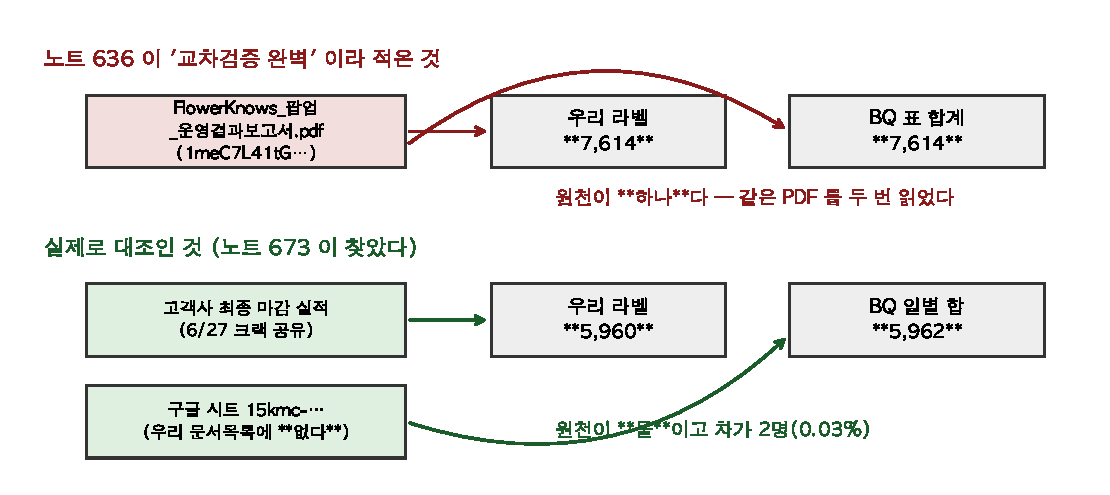
\includegraphics[width=0.98\textwidth]{figs/lineage.pdf}
\caption{위: 노트 636 의 ``교차검증''. 두 값이 같은 파일에서 나온다. 아래: 노트 673
이 찾은 진짜 대조. 우리 라벨은 고객사가 6/27 에 공유한 최종 마감 실적이고, 표는
\textbf{우리 문서목록에 없는} 구글 시트에서 왔다. 5{,}960 대 5{,}962 --- 차 2명.}
\end{figure}

\claim{노트 579·580 의 조항 \emph{`분자와 분모가 같은 것을 보는지 확인한다'} 가
\textbf{세 번째로} 발동했다. 앞의 둘은 축이 어긋났고(전이 4축 $\div$ 천장 5축) 표본이
어긋났다(통합=유보 $\rho$ $\div$ 전용=교차검증 최고점). 이번은 \textbf{원천}이
어긋났다 --- 두 수가 같은 파일에서 나오면 일치는 아무것도 안 말한다.}
{BQ 의 \texttt{source\_record\_id} 가 실제 원천을 안 가리키면(중간 단계 기록이면)
이 지적이 과할 수 있다. 다만 \texttt{RCPU2631} 에서는 그 필드가 우리 문서목록에
\emph{없는} 시트를 가리켰다 --- 필드가 원천을 구분하고 있다는 증거다.}

부수로 표의 의미도 확인됐다. \verb|total_visitor_count| $=$
\verb|actual_entry_count| $+$ \verb|walkin_count| 가 \textbf{47/48 행}에서 성립한다.
어긋난 한 행은 \verb|source_system='slack'| 이고 일별 내역 없이 총계만 있다 ---
결함이 아니라 출처가 다른 것이다. 그리고 \verb|reserved_count| 는 방문객이
\textbf{아니다}: \verb|RCPU2639| 는 예약 18{,}336 인데 방문 15{,}360 이다.

\section{흐름 --- 아직 흐르지 않는다}

\verb|created_at| 을 봤다. \textbf{48행 전부 2026-08-05 04:47$\sim$05:08 의 20분 창
안}이고, 그 뒤 \textbf{26시간 동안 한 행도 안 늘었다.}

\begin{figure}[t]\centering
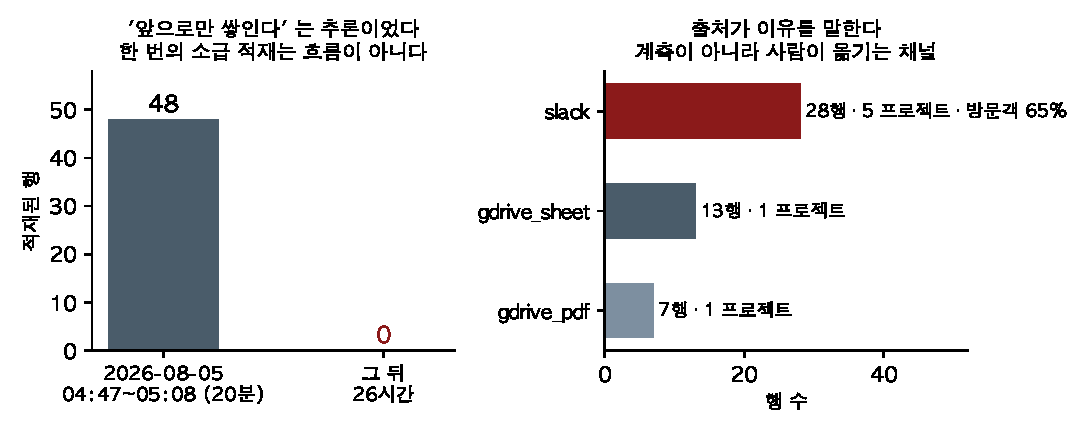
\includegraphics[width=0.98\textwidth]{figs/notflowing.pdf}
\caption{왼쪽: 단일 소급 적재. 오른쪽: 출처가 그 이유를 말한다 --- 48행 중
\textbf{28행(5 프로젝트 · 방문객의 65\%)이 \texttt{slack}} 이다.}
\end{figure}

\claim{이 표는 계측된 파이프라인이 아니라 \textbf{사람이 슬랙에 적은 것을 옮기는
채널}이다. 그러면 자라는 속도는 배관이 아니라 \textbf{사람의 습관}이 정한다 ---
26시간 증가 0의 유력한 설명이다. \textbf{한 번의 소급 적재는 흐름이 아니다.}}
{둘째 적재가 생기면 이 주장은 약해진다. 그래서 판정 조건을 미리 적었다: 새
\texttt{created\_at} 날짜가 하나라도 생기면 그때 월별 속도를 재고 배선을 판정한다.
\textbf{2주 안에 없으면 소급 적재 한 번으로 끝난 표}로 취급한다.}

\section{그래서 무엇이 달라지나}

\begin{itemize}
\item \textbf{T7 의 다음 실험이 근거를 잃었다.} 배선의 값은 ``앞으로 100\%''에
      기대고 있었고 그것이 아직 관측되지 않았다. 보류한다.
\item \textbf{학습 구간은 0행이다.} 표의 방문일이 전부 2026년이므로 판의 학습
      구간(2024)에 아무것도 안 더한다. 이건 내 예측대로였다 --- 다만
      \textbf{예측의 전제가 틀렸다.}
\item \textbf{그런데 표가 다른 것을 줬다.} 7 프로젝트 중 \textbf{4건은 레코드가
      아예 없다}(\verb|RCPU2637| 755 · \verb|RCPU2640| 1{,}556 ·
      \verb|RCPU2641| 6{,}305 · \verb|RCPU2642| 976). 그것은 \emph{라벨}이 아니라
      \textbf{행}이다. 내 사전등록은 ``라벨 없는 레코드가 몇인가''만 물었으므로
      \textbf{그 규칙에 사후로 끼워 넣지 않고} 별 항목으로 적었다.
\end{itemize}

그 4건이 다음 물음을 바꾼다. T7 은 줄곧 \emph{``어떻게 라벨을 더 캐나''}를 물었는데,
표가 보여 준 것은 \emph{``레코드 자체가 빠져 있다''}다. 다음 실험은
\verb|core.engagement|(578건)와 우리 레코드(380건)를 맞춰 \textbf{레코드가 없는
engagement 를 전수로 세는 것}이고, 판정은 ``그중 몇이 라벨·장소·날짜를 다 갖나''로
한다.

\section{사람이 정할 것 --- 쓰지 않았다}

\begin{itemize}
\item 새 라벨 \verb|RCPU2639| \textbf{15{,}360}(원천은 이 표 하나뿐이다).
\item 레코드가 없는 4건.
\item \textbf{\texttt{RCPU2631} 의 기간이 하루 어긋난다} --- 레코드는
      2026-06-11$\sim$06-24 인데 표의 방문일은 06-12$\sim$06-25 다(6/22 휴무 제외
      13일). 표에는 일별 실측이 있으므로 표가 옳을 가능성이 크다. 노트 552 가
      \emph{``날짜는 축 하나가 아니라 자를 만드는 것''}이라 적었으므로 이것은
      라벨보다 무겁다. \textbf{그래도 쓰지 않았다.}
\end{itemize}

\end{document}
